
%%%%%%%%%%%%%%%%%%%%%%%%%%%%%%%%%%%%%%%%%%%%%%%%%%%%%%%%%%%
%\emph{Human-swarm interaction results}\label{sec:expResults}
%%%%%%%%%%%%%%%%%%%%%%%%%%%%%%%%%%%%%%%%%%%%%%%%%%%%%%%%%%%

We designed six experiments to investigate human control of large swarms for manipulation tasks.  Screenshots of representative experiments are shown in Fig.~\ref{fig:5experiments}.  Each experiment examined the effects of varying a single parameter: population of particles for manipulation, four levels of visual feedback, different levels of Brownian noise.  %, position control with 1 to 10 particles, and three control architectures for both assembly and foraging tasks. 
 The users could choose which experiment to try, and our architecture randomly assigned a parameter value for each trial.  We recorded the completion time and the participant ID for each successful trial.  
%As Fig.~\ref{fig:Learning} shows, one-third of all participants played only a single game.  Still, many played multiple games, and their decreasing completion times demonstrates their skills improved.


\subsection{Varying number}
\begin{figure}
\begin{overpic}[width = 0.9\columnwidth]{ResVaryNum.pdf}\end{overpic}
%\begin{overpic}[width = 0.48\columnwidth]{measureLearning.pdf}\end{overpic}
\caption{
\label{fig:ResVaryNu}Data from \emph{Varying Number} using particles to push an object through a maze to a goal location. 
% Best-fit linear and quadratic lines are overlaid for comparison. 
%(Right) Skill improves as players retry tests using data from \emph{Varying Number}.
}
\end{figure}



%Transport of goods and materials between points is at the heart of all engineering and construction in real-world systems. 
This experiment varied from 1 to 500 the population of particles used to transport an object. The total area, maximum particle speed, and total net force the swarm could produce were constant. The particles pushed a large hexagonal object through an  {\sffamily S}-shaped maze. We hypothesized participants would complete the task faster with more particles. The results, shown in Fig.~\ref{fig:ResVaryNu}, do not support our hypothesis, indicating a minimum around 130 particles, but only a gradual increase in completion time from 50 to 500.


\subsection{Varying visualization}
\begin{figure}[b!]
\renewcommand{\figwid}{0.24\columnwidth}
\begin{overpic}[width =\figwid]{VaryVisFS.pdf}\put(20,15){Full-state}\end{overpic}
\begin{overpic}[width =\figwid]{VaryVisCH.pdf}\put(10,15){Convex-hull}\end{overpic}
\begin{overpic}[width =\figwid]{VaryVisMV.pdf}\put(10,15){Mean + var}\end{overpic}
\begin{overpic}[width =\figwid]{VaryVisMe.pdf}\put(30,15){Mean}\end{overpic}
\vspace{-.5em}
\caption{\label{fig:Visualization}Screenshots from task \emph{Vary Visualization}. This experiment challenges players to quickly steer 100 particles (blue discs) to push an object (green hexagon) into a goal region. We record the completion time and other statistics.
%\vspace{-1em}
}
\end{figure}

\begin{figure}
%  \vspace{-20pt}
  \begin{center}
  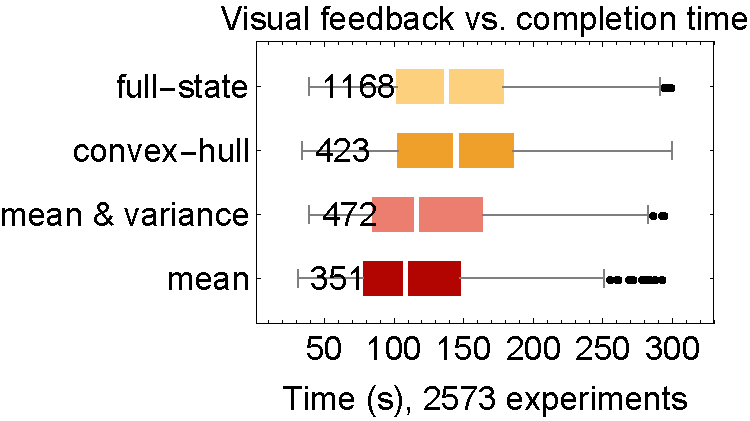
\includegraphics[width=0.8\columnwidth]{ResVaryVis.pdf}
  \end{center}
%  \vspace{-1em}
\caption{\label{fig:ResVaryVis} Completion-time results for the four levels of visual feedback shown in Fig.~\ref{fig:Visualization}.  Players performed better with limited feedback.
\vspace{-1em}
}
\end{figure}

%Sensing is expensive, especially on the nanoscale. To see nanocars~\cite{Chiang2011} fastened molecules that fluoresce light when activated by a strong light source. 
%Unfortunately, multiple exposures can destroy these molecules, a process called \emph{photobleaching}. 
%Photobleaching can be minimized by lowering the excitation light intensity, but \cite{Cazes2001} showed this increases the probability of missed detections.  
This experiment explores manipulation with varying amounts of sensing information: {\bf full-state} sensing provides the most information by showing the position of all particles; {\bf convex-hull} draws a convex hull around the outermost particles; {\bf mean} provides the average position of the population; and {\bf mean + variance} adds a confidence ellipse. Fig.~\ref{fig:Visualization} shows screenshots of the same particle swarm with each type of visual feedback. Full-state requires $2n$ data points for $n$ particles. Convex-hull requires at worst $2n$, but according to Har \cite{har2011expected}, the expected number is $O(2 n^{1/3})$.  Mean requires two, and variance three, data points.  Because they do not increase with population size, mean and mean + variance are convenient even with millions of particles. 



Our hypothesis predicted a steady decrease in performance as the amount of visual feedback decreased.
Our experiment indicated the opposite: players with just the mean completed the task faster than those with full-state feedback.  As Fig.~\ref{fig:ResVaryVis} shows, the levels of feedback arranged by increasing completion time are [mean, mean + variance, full-state, convex-hull].  All experiments lasting over 300 s were removed, under the assumption that the user stopped playing. 
Using ANOVA analysis, we rejected the null hypothesis that all visualization methods are equivalent, with $p$-value $2.69\times10^{-19}$.
Anecdotal evidence from beta-testers who played the game suggests that tracking 100 particles is overwhelming---similar to schooling phenomenons that confuse predators---while working with just the mean + variance is like using a ``spongy'' manipulator. However, our beta-testers described convex-hull feedback as confusing and irritating since it is not robust to outliers.  A single particle left behind an obstacle will stretch the entire hull, obscuring the majority of the swarm.
%obscuring what the rest of the swarm is doing.   

\begin{figure}[b!]
\renewcommand{\figwid}{0.49\columnwidth}
\begin{overpic}[width =\figwid]{ResVaryNoise.pdf}\end{overpic}
\begin{overpic}[width =\figwid]{ResPositioning.pdf}\end{overpic}
%\vspace{-1em}
\caption{\label{fig:ResVaryNoisePosition} Left: Varying the noise from 0 to 200\% of the maximum control input resulted in only a small increase in completion time. Right: For position control, increasing the number of particles resulted in longer completion times.  For more than 4 particles the goal pattern contained a void, which may have caused the jump in completion times.
%\vspace{-1em}
}
\end{figure}

\subsection{Varying noise}
%Micro-particles are affected by random collisions with molecules. The effect of these collisions is called Brownian motion.
This experiment varied the strength of %these 
disturbances to study how noise (disturbance inputs) affects human control of large swarms. Noise was applied at every time step as follows:
\begin{align*}
\dot{x}_i &= u_x + m_i\cos(\psi_i)\\
 \dot{y}_i &= u_y + m_i\sin(\psi_i).
 \end{align*}
Here, $m_i$ and $\psi_i$ were uniformly IID, with $m_i\in[0,M]$ and $\psi_i\in[0,2\pi]$. $M$ was a constant for each trial ranging from 0 to 200\% of the maximum control power ($u_{\rm{max}}$).
 
We hypothesized 200\% noise was the largest a human could be expected to control---at 200\% noise, the particles move erratically.  Disproving our hypothesis, the results in Fig.~\ref{fig:ResVaryNoisePosition}a show only a 40\% increase in completion time for the maximum noise. This indicates swarm control is robust to IID noise.


